\subsection{Datasets} \label{subsec:datasets}

We evaluate on three datasets: a multi-dimensional synthetic set, a 2D diverse synthetic set, and the EUC\_2D subset of TSPLIB95. The synthetic sets are held-out test splits from our generation pipeline (Appendix~\ref{app:training}); TSPLIB95 is real-world. The evaluation pipeline assumes symmetric metric distances; instances that violate the triangle inequality (e.g.\ the bridge-graph outlier \texttt{brg180}) are excluded from every aggregate.

\subsubsection{Multi-dimensional synthetic ($d = 2$--$100$)}
16{,}907 held-out instances with $n \in [5, 1000]$ and $d \in \{2, 3, \ldots, 50, 100\}$, sampled by stratified dimension--size--grid buckets across 16 per-dimension distribution types drawn from the generators used for our training set: uniform, normal, clustered ($k$-means \citep{lloyd1982}), and autoregressive-correlated. Stratification enforces zero overlap with the training split. $d = 100$ is outside the training range and serves as the extrapolation test.

\subsubsection{2D diverse synthetic}
2{,}580 instances, $d = 2$, $n \in [5, 1000]$, coordinate grid side-length $G \in [1000, 10000]$. Five distribution classes (Table~\ref{tab:dataset_counts}) each probe a different assumption made by classical 2D estimators. Four classes (isotropic, biased, geometric, clustered) follow conventions used in the TSP-instance-generation literature, including the variants reported by \citet{cavdar2015distribution} for the distribution-free baseline. The fifth class, \textit{Line Noise}, generates near-linear manifolds of the form $y = mx + b + \epsilon$ with small $\epsilon$. This geometry is \emph{not} represented in the training distribution: we include it precisely to measure how the model handles point sets that collapse toward a 1D manifold, where hull-based formulas vanish and bounding-box formulas over-predict.

\begin{table}[!ht]
\centering
\caption{2D benchmark dataset composition (2{,}580 instances).}
\label{tab:dataset_counts}
\resizebox{\textwidth}{!}{%
\begin{tabular}{@{}llcp{6cm}@{}}
\toprule
\textbf{Class} & \textbf{Generators} & \textbf{Count} & \textbf{Stress target} \\ \midrule
Isotropic Noise & Uniform, Normal, Triangular, Truncated Exp. & 840 & Control: $A_{\text{hull}} \approx A_{\text{box}}$. \\
Biased / Skewed & Squeezed, Uni-Tri, Tri-Squeezed, Correlated & 840 & Aspect-ratio distortion: $\sigma_x \neq \sigma_y$. \\
Geometric Struct. & Grid, Boundary (hollow), X-Central & 630 & Lattice regularity, hollow voids. \\
Clustered & $k$-Means ($k \in [5, 20]$) & 60 & Bimodal edge-weight distribution. \\
Line Noise\textsuperscript{$\dagger$} & Linear manifold $y=mx+b+\epsilon$ & 210 & Hull/box divergence as data collapses toward 1D. \\ \midrule
\textbf{Total} & & \textbf{2{,}580} & \\
\bottomrule
\multicolumn{4}{l}{\footnotesize $^{\dagger}$ Not represented in training; included to measure generalization to unseen geometries.}
\end{tabular}%
}
\end{table}

\subsubsection{TSPLIB95 EUC\_2D common subset}
78 EUC\_2D instances with $n$ from 14 to 85{,}900 \citep{reinelt1991tsplib}. This is the intersection where every benchmark model is directly applicable: all classical baselines require 2D Euclidean coordinates, and the MST Ratio baseline needs only a distance matrix. The remaining 32 metric TSPLIB95 instances (CEIL\_2D, ATT pseudo-Euclidean, GEO great-circle, EXPLICIT-metric) are not natively Euclidean and are evaluated in Section~\ref{sec:application} via MDS embedding, which only GART 2.0 supports. For large instances where the dense $n \times n$ distance matrix would exceed memory, we replace it with a Delaunay-based MST construction \citep{delaunay1934} that uses only $O(n)$ edges.

\subsection{Results} \label{subsec:results}

Every table below reports the same seven quantities per model: instance count $N$, MAPE, SDPE, median $|\%\,\text{error}|$, $R^2$ on tour cost, $R^2_\alpha$ on the MST--TSP ratio (only where the model predicts $\alpha$ directly), and mean total prediction time in milliseconds (feature extraction + MST + inference).

\subsubsection{Multi-dimensional benchmark} \label{subsec:results_nd}

We present the 16{,}907-instance multi-dimensional benchmark in two orthogonal slices: by instance size (Table~\ref{tab:nd_by_size}) and by dimension (Table~\ref{tab:nd_by_dim}). Both tables summarize the same underlying data.

\begin{table}[!ht]
\centering
\caption{ND benchmark by instance size. Same 16{,}907 instances as Table~\ref{tab:nd_by_dim}.}
\label{tab:nd_by_size}
\resizebox{\textwidth}{!}{%
\footnotesize
\begin{tabular}{@{}ll rrrrrrr@{}}
\toprule
$n$ bucket & Model & $N$ & MAPE (\%) & SDPE (\%) & Median (\%) & $R^2$ & $R^2_\alpha$ & Time (ms) \\
\midrule
    \multirow{3}{*}{$[5,10]$}
    & GART 2.0 & 4{,}227 & \textbf{1.36} & \textbf{1.90} & 0.99 & 1.000 & 0.943 & 211 \\
    & MST Ratio & 4{,}227 & 18.89 & 5.44 & 17.89 & 0.966 & $-4.631$ & 13.3 \\
    & Hilbert & 4{,}227 & 8.11 & 7.45 & 5.75 & 0.995 & --- & 31.3 \\
    \midrule
    \multirow{3}{*}{$[11,50]$}
    & GART 2.0 & 2{,}816 & \textbf{0.88} & \textbf{1.17} & 0.73 & 1.000 & 0.928 & 235 \\
    & MST Ratio & 2{,}816 & 7.45 & 2.89 & 6.94 & 0.997 & $-2.077$ & 34.5 \\
    & Hilbert & 2{,}816 & 19.59 & 12.35 & 15.60 & 0.981 & --- & 75.7 \\
    \midrule
    \multirow{3}{*}{$[51,100]$}
    & GART 2.0 & 3{,}522 & \textbf{0.66} & \textbf{0.79} & 0.58 & 1.000 & 0.950 & 271 \\
    & MST Ratio & 3{,}522 & 5.33 & 2.13 & 4.80 & 0.998 & $-1.371$ & 56.8 \\
    & Hilbert & 3{,}522 & 24.38 & 14.10 & 20.18 & 0.973 & --- & 147 \\
    \midrule
    \multirow{3}{*}{$[101,200]$}
    & GART 2.0 & 703 & \textbf{0.55} & \textbf{0.63} & 0.47 & 1.000 & 0.958 & 338 \\
    & MST Ratio & 703 & 4.44 & 1.74 & 4.12 & 0.999 & $-1.103$ & 95.0 \\
    & Hilbert & 703 & 27.03 & 13.61 & 23.40 & 0.965 & --- & 311 \\
    \midrule
    \multirow{3}{*}{$[201,500]$}
    & GART 2.0 & 2{,}115 & \textbf{0.50} & \textbf{0.56} & 0.39 & 1.000 & 0.956 & 388 \\
    & MST Ratio & 2{,}115 & 4.06 & 1.51 & 3.80 & 0.999 & $-1.097$ & 152 \\
    & Hilbert & 2{,}115 & 28.26 & 12.75 & 26.22 & 0.960 & --- & 477 \\
    \midrule
    \multirow{3}{*}{$[501,1000]$}
    & GART 2.0 & 3{,}524 & \textbf{0.48} & \textbf{0.55} & 0.31 & 1.000 & 0.949 & 570 \\
    & MST Ratio & 3{,}524 & 3.82 & 1.32 & 3.63 & 0.999 & $-1.134$ & 426 \\
    & Hilbert & 3{,}524 & 29.97 & 12.77 & 28.71 & 0.953 & --- & 2056 \\
    \midrule
    \multirow{3}{*}{\textbf{ALL}}
    & \textbf{GART 2.0} & \textbf{16{,}907} & \textbf{0.81} & \textbf{1.17} & \textbf{0.63} & \textbf{1.000} & \textbf{0.978} & \textbf{330} \\
    & MST Ratio & 16{,}907 & 8.56 & 6.89 & 5.61 & 0.999 & $-0.834$ & 133 \\
    & Hilbert & 16{,}907 & 21.28 & 14.55 & 16.22 & 0.962 & --- & 552 \\
\bottomrule
\end{tabular}%
}
\end{table}

\begin{table}[!ht]
\centering
\caption{ND benchmark by dimension. Same 16{,}907 instances as Table~\ref{tab:nd_by_size}. $d = 100$ is outside the training range (extrapolation).}
\label{tab:nd_by_dim}
\resizebox{\textwidth}{!}{%
\footnotesize
\begin{tabular}{@{}ll rrrrrrr@{}}
\toprule
$d$ bucket & Model & $N$ & MAPE (\%) & SDPE (\%) & Median (\%) & $R^2$ & $R^2_\alpha$ & Time (ms) \\
\midrule
    \multirow{3}{*}{$d=2$}
    & GART 2.0 & 647 & \textbf{1.82} & \textbf{2.75} & 0.99 & 1.000 & 0.955 & 317 \\
    & MST Ratio & 647 & 13.19 & 10.70 & 8.95 & 0.995 & $-0.983$ & 98.0 \\
    & Hilbert & 647 & 30.36 & 16.41 & 35.31 & 0.804 & --- & 82.8 \\
    \midrule
    \multirow{3}{*}{$d=3$--$5$}
    & GART 2.0 & 1{,}941 & \textbf{1.16} & \textbf{1.83} & 0.64 & 1.000 & 0.962 & 319 \\
    & MST Ratio & 1{,}941 & 11.72 & 8.07 & 8.02 & 0.996 & $-1.376$ & 97.6 \\
    & Hilbert & 1{,}941 & 35.53 & 15.82 & 39.96 & 0.737 & --- & 105 \\
    \midrule
    \multirow{3}{*}{$d=6$--$10$}
    & GART 2.0 & 3{,}240 & \textbf{0.83} & \textbf{1.28} & 0.48 & 1.000 & 0.971 & 323 \\
    & MST Ratio & 3{,}240 & 10.27 & 6.64 & 7.19 & 0.997 & $-1.674$ & 103 \\
    & Hilbert & 3{,}240 & 32.78 & 14.34 & 36.20 & 0.789 & --- & 157 \\
    \midrule
    \multirow{3}{*}{$d=15$--$25$}
    & GART 2.0 & 1{,}944 & \textbf{0.55} & \textbf{0.84} & 0.31 & 1.000 & 0.984 & 328 \\
    & MST Ratio & 1{,}944 & 8.72 & 6.02 & 5.70 & 0.998 & $-1.570$ & 114 \\
    & Hilbert & 1{,}944 & 24.73 & 11.81 & 26.33 & 0.846 & --- & 295 \\
    \midrule
    \multirow{3}{*}{$d=30$--$50$}
    & GART 2.0 & 3{,}236 & \textbf{0.36} & \textbf{0.58} & 0.20 & 1.000 & 0.992 & 330 \\
    & MST Ratio & 3{,}236 & 7.63 & 5.90 & 4.60 & 0.999 & $-1.300$ & 127 \\
    & Hilbert & 3{,}236 & 17.14 & 7.98 & 18.13 & 0.924 & --- & 494 \\
    \midrule
    \multirow{3}{*}{$d=100^{*}$}
    & GART 2.0 & 5{,}899 & \textbf{0.90} & \textbf{0.50} & 0.89 & 1.000 & 0.980 & 339 \\
    & MST Ratio & 5{,}899 & 6.54 & 5.93 & 3.43 & 0.999 & $-0.995$ & 173 \\
    & Hilbert & 5{,}899 & 10.40 & 4.60 & 11.08 & 0.971 & --- & 1084 \\
    \midrule
    \multirow{3}{*}{\textbf{ALL}}
    & \textbf{GART 2.0} & \textbf{16{,}907} & \textbf{0.81} & \textbf{1.17} & \textbf{0.63} & \textbf{1.000} & \textbf{0.978} & \textbf{330} \\
    & MST Ratio & 16{,}907 & 8.56 & 6.89 & 5.61 & 0.999 & $-0.834$ & 133 \\
    & Hilbert & 16{,}907 & 21.28 & 14.55 & 16.22 & 0.962 & --- & 552 \\
\bottomrule
\multicolumn{9}{l}{\footnotesize $^{*}$ $d = 100$ is outside the training range; included to test extrapolation.}
\end{tabular}%
}
\end{table}

\begin{figure}[!ht]
\centering
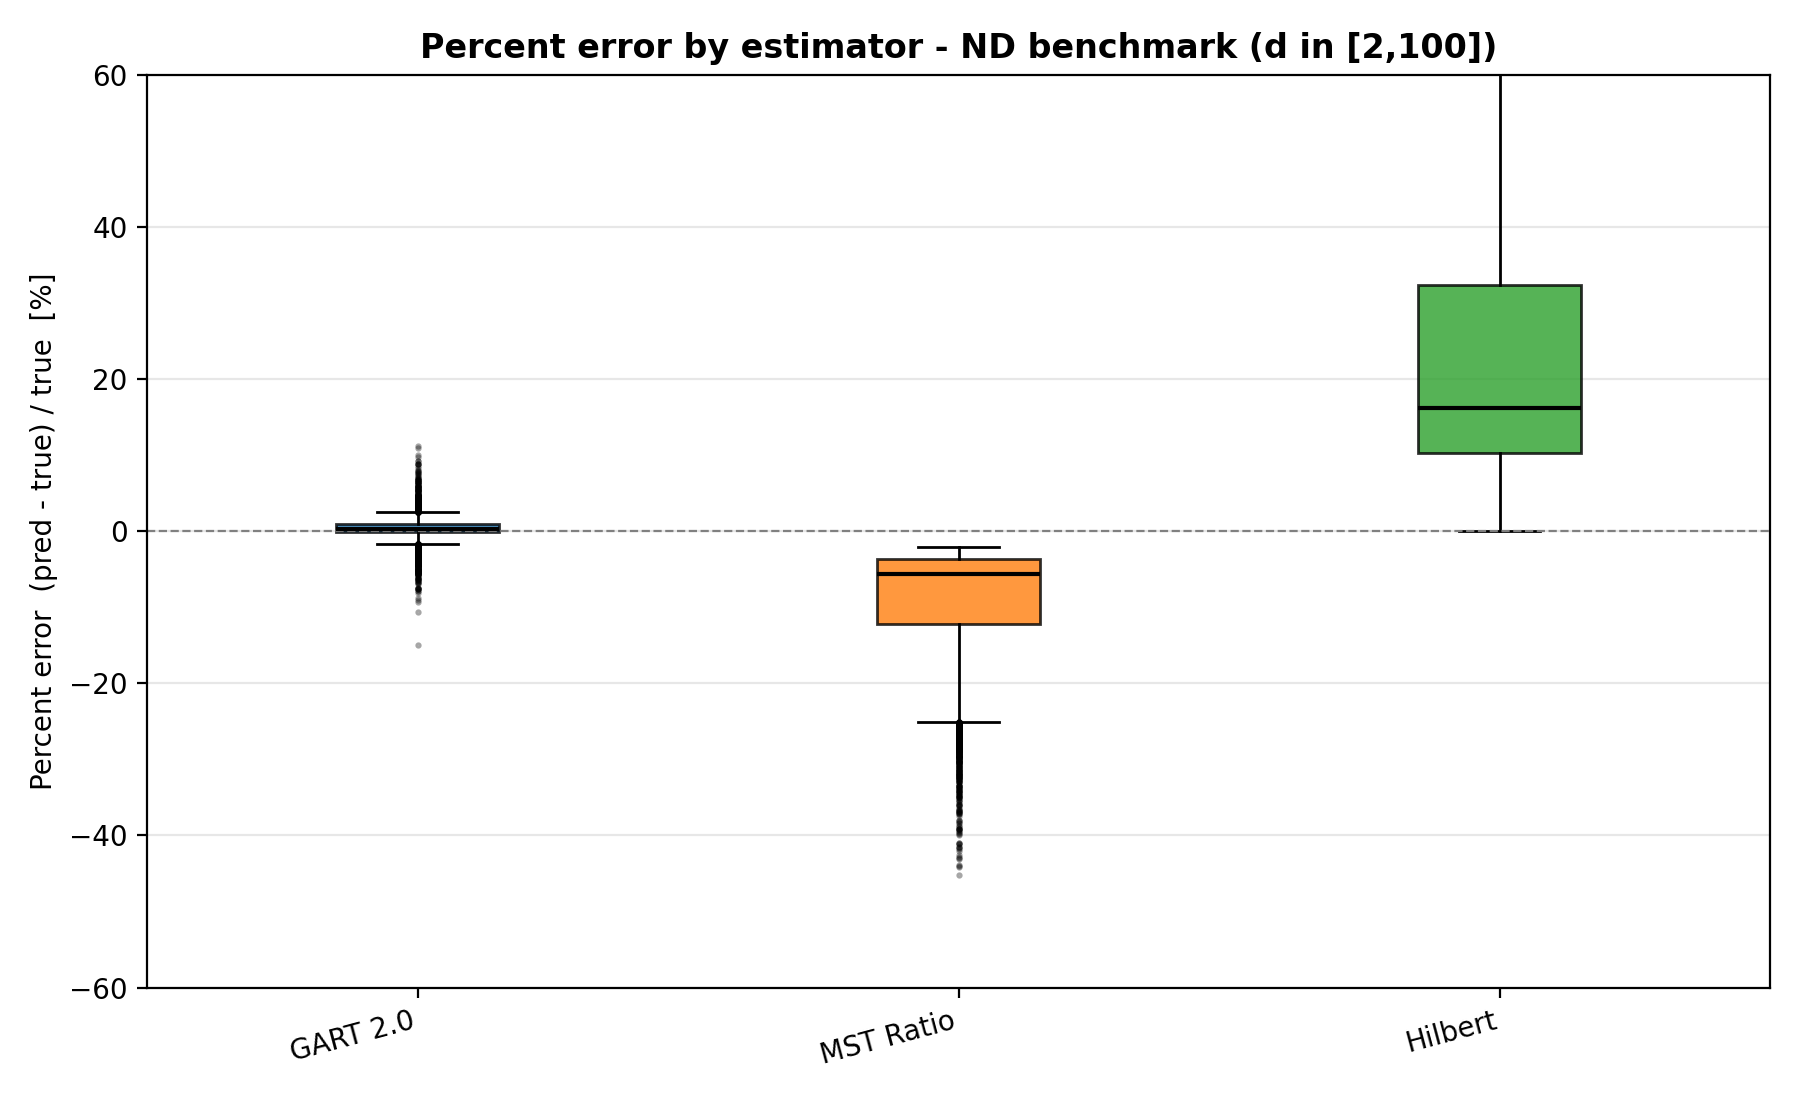
\includegraphics[width=0.75\textwidth]{boxplot_nd_errors.png}
\caption{Percent-error distribution per model on the ND benchmark (16{,}907 instances).}
\label{fig:boxplot_nd}
\end{figure}

GART 2.0 reaches 0.81\% MAPE and 1.17\% SDPE overall, against 8.56\% / 6.89\% for MST Ratio and 21.28\% / 14.55\% for Hilbert. Precision tightens monotonically as $n$ grows (SDPE drops from 1.90\% at $n \le 10$ to 0.55\% at $n \ge 500$) and as $d$ grows (2.75\% at $d = 2$ down to 0.50\% at $d = 100$), consistent with the theoretical convergence $\alpha \to 1$ in high dimensions \citep{percus1996}. MST Ratio's SDPE is nearly flat because its fixed constant does not adapt to instance structure. Hilbert degrades with $n$ because space-filling locality breaks on non-uniform distributions.

\subsubsection{2D diverse benchmark} \label{subsec:results_2d}

Table~\ref{tab:2d_by_size} disaggregates the 2{,}580-instance 2D benchmark by instance size.

\begin{table}[!ht]
\centering
\caption{2D diverse benchmark by instance size (2{,}580 instances). $R^2_\alpha$ is computed per bucket; it is only defined for models that predict $\alpha$ directly.}
\label{tab:2d_by_size}
\resizebox{\textwidth}{!}{%
\footnotesize
\begin{tabular}{@{}ll rrrrrrr@{}}
\toprule
$n$ bucket & Model & $N$ & MAPE (\%) & SDPE (\%) & Median (\%) & $R^2$ & $R^2_\alpha$ & Time (ms) \\
\midrule
    \multirow{6}{*}{$[5,10]$}
    & GART 2.0 & 360 & \textbf{4.53} & \textbf{5.53} & 3.80 & 0.993 & 0.846 & 132 \\
    & MST Ratio & 360 & 28.95 & 9.99 & 29.17 & 0.785 & $-4.777$ & 9.84 \\
    & Cavdar & 360 & 17.37 & 14.25 & 13.18 & 0.904 & --- & 6.67 \\
    & BHH & 360 & 59.32 & 9.74 & 57.70 & 0.203 & --- & 7.81 \\
    & Chien & 360 & 25.81 & 7.23 & 26.24 & 0.842 & --- & 1.14 \\
    & Hilbert & 360 & 8.35 & 8.84 & 5.79 & 0.965 & --- & 3.63 \\
    \midrule
    \multirow{6}{*}{$[11,50]$}
    & GART 2.0 & 480 & \textbf{4.18} & \textbf{5.87} & 2.77 & 0.994 & 0.730 & 133 \\
    & MST Ratio & 480 & 15.16 & 9.66 & 13.63 & 0.949 & $-1.461$ & 15.2 \\
    & Cavdar & 480 & 12.73 & 16.28 & 8.45 & 0.943 & --- & 8.85 \\
    & BHH & 480 & 28.38 & 9.28 & 27.64 & 0.817 & --- & 8.94 \\
    & Chien & 480 & 19.64 & 18.68 & 17.88 & 0.888 & --- & 1.29 \\
    & Hilbert & 480 & 27.18 & 10.37 & 26.95 & 0.804 & --- & 3.04 \\
    \midrule
    \multirow{6}{*}{$[51,100]$}
    & GART 2.0 & 630 & \textbf{3.57} & \textbf{5.53} & 2.05 & 0.995 & 0.666 & 173 \\
    & MST Ratio & 630 & 11.45 & 8.59 & 9.34 & 0.975 & $-1.012$ & 29.4 \\
    & Cavdar & 630 & 19.07 & 29.40 & 7.45 & 0.897 & --- & 8.59 \\
    & BHH & 630 & 16.22 & 13.08 & 14.98 & 0.912 & --- & 11.0 \\
    & Chien & 630 & 23.38 & 30.74 & 16.69 & 0.853 & --- & 0.56 \\
    & Hilbert & 630 & 34.23 & 9.82 & 34.08 & 0.734 & --- & 3.87 \\
    \midrule
    \multirow{6}{*}{$[101,200]$}
    & GART 2.0 & 120 & \textbf{2.86} & \textbf{5.03} & 1.30 & 0.996 & 0.560 & 196 \\
    & MST Ratio & 120 & 8.31 & 7.06 & 6.72 & 0.989 & $-0.775$ & 32.7 \\
    & Cavdar & 120 & 18.70 & 41.03 & 3.36 & 0.911 & --- & 7.86 \\
    & BHH & 120 & 11.82 & 20.23 & 6.85 & 0.946 & --- & 10.2 \\
    & Chien & 120 & 25.75 & 42.94 & 15.23 & 0.853 & --- & 0.30 \\
    & Hilbert & 120 & 36.61 & 10.48 & 36.48 & 0.717 & --- & 7.39 \\
    \midrule
    \multirow{6}{*}{$[201,500]$}
    & GART 2.0 & 380 & \textbf{2.48} & \textbf{4.22} & 1.14 & 0.997 & 0.564 & 215 \\
    & MST Ratio & 380 & 7.19 & 6.04 & 5.94 & 0.992 & $-0.857$ & 82.9 \\
    & Cavdar & 380 & 26.11 & 55.60 & 3.21 & 0.867 & --- & 14.3 \\
    & BHH & 380 & 15.35 & 32.05 & 4.26 & 0.927 & --- & 9.72 \\
    & Chien & 380 & 30.90 & 56.03 & 14.49 & 0.823 & --- & 5.74 \\
    & Hilbert & 380 & 38.59 & 9.94 & 38.21 & 0.717 & --- & 39.0 \\
    \midrule
    \multirow{6}{*}{$[501,1000]$}
    & GART 2.0 & 610 & \textbf{1.92} & \textbf{3.16} & 0.95 & 0.997 & 0.550 & 424 \\
    & MST Ratio & 610 & 5.71 & 4.54 & 5.00 & 0.994 & $-0.994$ & 237 \\
    & Cavdar & 610 & 23.93 & 58.54 & 3.39 & 0.872 & --- & 25.3 \\
    & BHH & 610 & 14.75 & 33.64 & 5.08 & 0.931 & --- & 15.9 \\
    & Chien & 610 & 29.90 & 59.34 & 14.07 & 0.823 & --- & 14.0 \\
    & Hilbert & 610 & 38.24 & 11.17 & 38.21 & 0.728 & --- & 93.9 \\
    \midrule
    \multirow{6}{*}{\textbf{ALL}}
    & \textbf{GART 2.0} & \textbf{2{,}580} & \textbf{3.23} & \textbf{4.94} & \textbf{1.73} & \textbf{0.998} & \textbf{0.861} & \textbf{226} \\
    & MST Ratio & 2{,}580 & 12.45 & 11.06 & 8.16 & 0.992 & $-0.766$ & 81.1 \\
    & Cavdar & 2{,}580 & 19.82 & 42.04 & 6.13 & 0.909 & --- & 13.1 \\
    & BHH & 2{,}580 & 23.82 & 32.05 & 15.55 & 0.943 & --- & 11.1 \\
    & Chien & 2{,}580 & 25.78 & 42.55 & 17.25 & 0.874 & --- & 4.71 \\
    & Hilbert & 2{,}580 & 31.01 & 14.24 & 34.99 & 0.801 & --- & 30.3 \\
\bottomrule
\end{tabular}%
}
\end{table}

\begin{figure}[!ht]
\centering
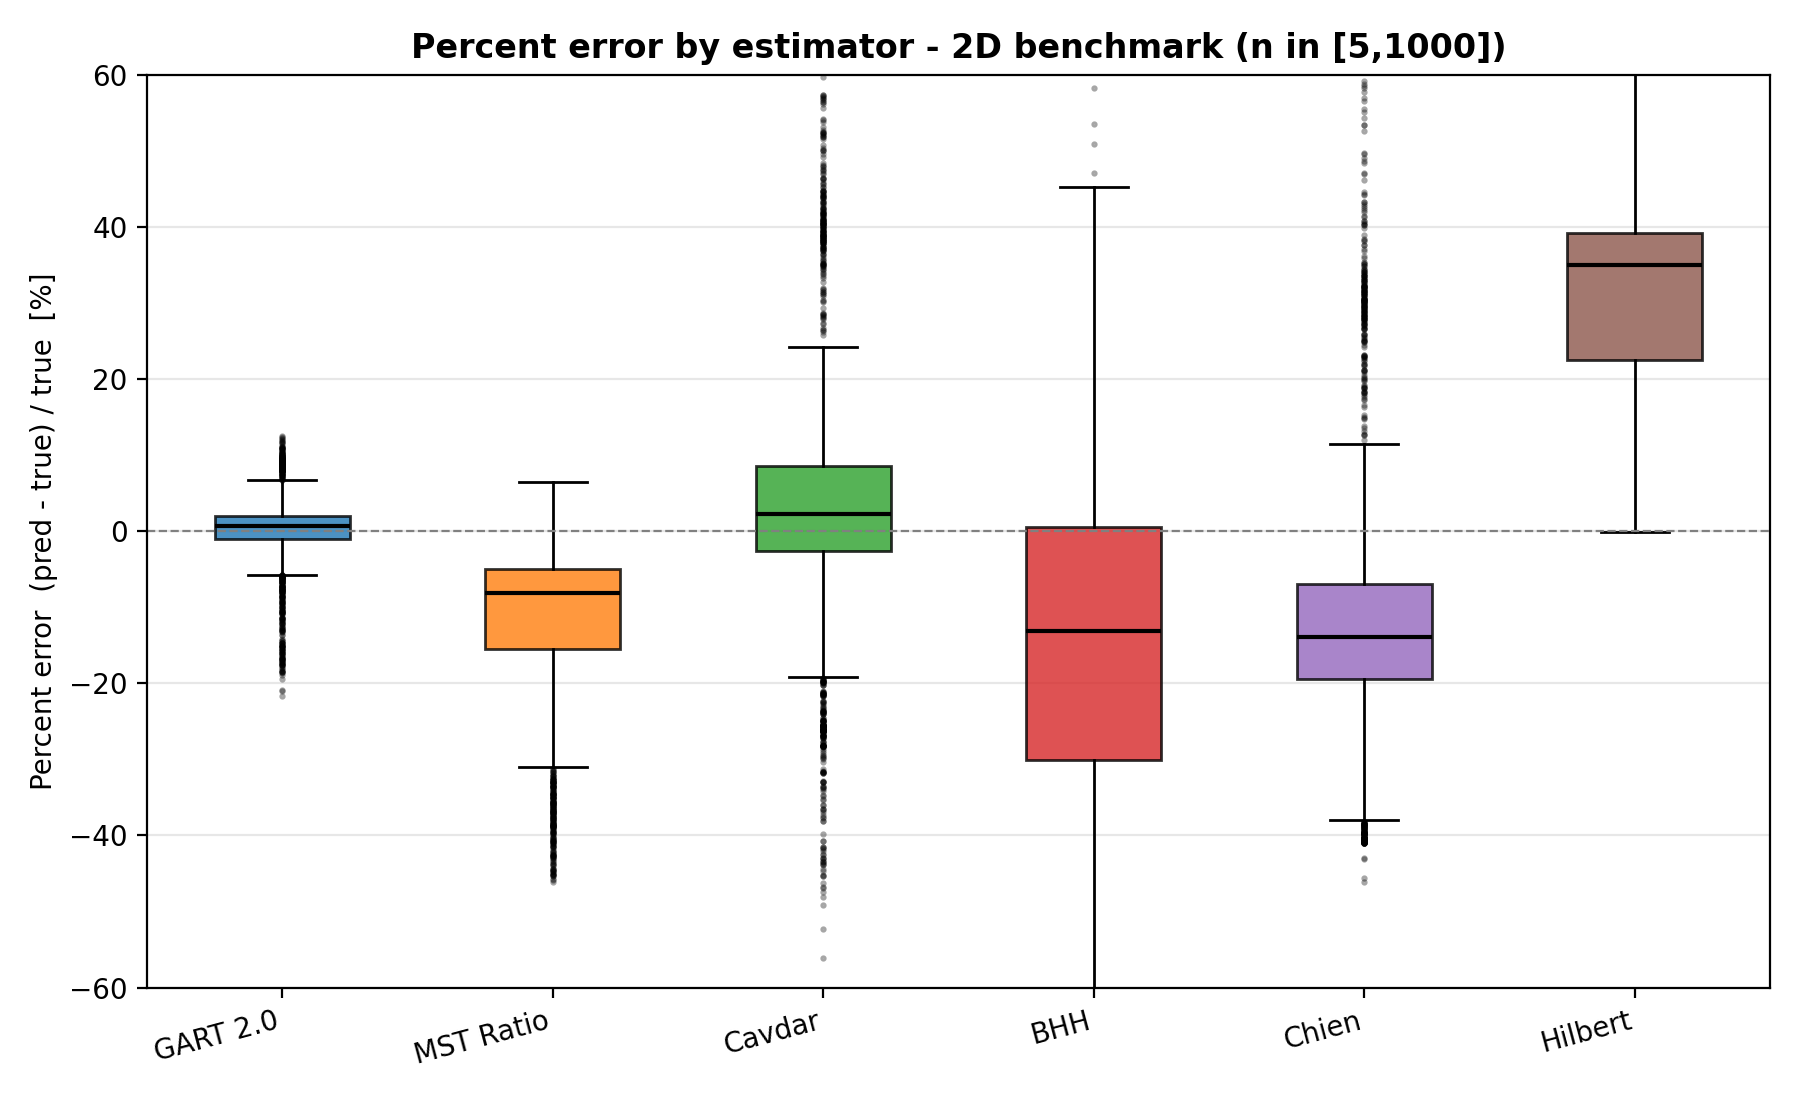
\includegraphics[width=0.75\textwidth]{boxplot_2d_errors.png}
\caption{Percent-error distribution per model on the 2D diverse benchmark (2{,}580 instances).}
\label{fig:boxplot_2d}
\end{figure}

GART 2.0 leads at 3.23\% MAPE / 4.94\% SDPE overall. MST Ratio is second at 12.45\% / 11.06\%. Cavdar, BHH, and Chien exceed 30\% SDPE because their enclosure-based formulas amplify variance on the Biased and Line Noise classes, where bounding-box and hull volumes diverge. Hilbert has intermediate MAPE (31\%) but lower SDPE (14\%): its errors are large but consistent --- a systematic space-filling bias. GART's per-bucket $R^2_\alpha$ drops from 0.85 at $n \le 10$ to 0.55 at mid-size buckets, reflecting two things: smaller buckets have wider true-$\alpha$ variance (easier to explain), and the diverse-distribution stresses bring $\alpha$ closer to 1.07--1.15 at larger $n$, where small prediction errors consume proportionally more variance.

\subsubsection{TSPLIB95 EUC\_2D benchmark} \label{subsec:results_tsplib}

Table~\ref{tab:tsplib_by_size} reports per-size-bucket results across all 78 EUC\_2D instances, with $n$ from 14 to 85{,}900.

\begin{table}[!ht]
\centering
\caption{TSPLIB95 EUC\_2D benchmark by instance size (78 instances).}
\label{tab:tsplib_by_size}
\resizebox{\textwidth}{!}{%
\footnotesize
\begin{tabular}{@{}ll rrrrrrr@{}}
\toprule
$n$ bucket & Model & $N$ & MAPE (\%) & SDPE (\%) & Median (\%) & $R^2$ & $R^2_\alpha$ & Time (ms) \\
\midrule
    \multirow{6}{*}{$[51,150]$}
    & GART 2.0 & 23 & \textbf{2.83} & \textbf{3.28} & 1.71 & 0.996 & 0.301 & 9.33 \\
    & MST Ratio & 23 & 6.93 & 4.05 & 6.12 & 0.978 & $-2.609$ & 0.93 \\
    & Cavdar & 23 & 10.00 & 14.37 & 6.44 & 0.936 & --- & 0.71 \\
    & BHH & 23 & 16.09 & 15.99 & 13.59 & 0.958 & --- & 0.73 \\
    & Chien & 23 & 18.45 & 14.58 & 17.84 & 0.948 & --- & 0.11 \\
    & Hilbert & 23 & 39.91 & 11.46 & 38.92 & 0.757 & --- & 0.72 \\
    \midrule
    \multirow{6}{*}{$[151,500]$}
    & GART 2.0 & 20 & \textbf{3.29} & \textbf{3.68} & 2.66 & 0.997 & 0.298 & 17.7 \\
    & MST Ratio & 20 & 6.10 & 4.88 & 5.00 & 0.986 & $-1.297$ & 6.83 \\
    & Cavdar & 20 & 23.20 & 29.75 & 12.33 & 0.588 & --- & 0.69 \\
    & BHH & 20 & 20.48 & 29.65 & 7.38 & 0.776 & --- & 0.93 \\
    & Chien & 20 & 24.02 & 29.72 & 18.98 & 0.854 & --- & 0.15 \\
    & Hilbert & 20 & 44.44 & 7.64 & 42.42 & 0.492 & --- & 1.82 \\
    \midrule
    \multirow{6}{*}{$[501,2000]$}
    & GART 2.0 & 21 & \textbf{3.39} & \textbf{3.57} & 2.17 & 0.999 & $-0.750$ & 37.1 \\
    & MST Ratio & 21 & 4.40 & 3.48 & 5.30 & 0.993 & $-1.294$ & 177 \\
    & Cavdar & 21 & 31.48 & 41.61 & 16.16 & 0.806 & --- & 1.31 \\
    & BHH & 21 & 35.95 & 49.39 & 15.53 & 0.809 & --- & 1.66 \\
    & Chien & 21 & 29.55 & 44.34 & 16.72 & 0.954 & --- & 0.58 \\
    & Hilbert & 21 & 51.18 & 11.02 & 49.11 & 0.265 & --- & 8.14 \\
    \midrule
    \multirow{6}{*}{$[2001,10000]$}
    & GART 2.0 & 9 & \textbf{5.77} & \textbf{3.49} & 5.02 & 0.992 & $-2.317$ & 51.0 \\
    & MST Ratio & 9 & 2.70 & 3.76 & 1.96 & 0.999 & $-0.000$ & 882 \\
    & Cavdar & 9 & 39.58 & 67.84 & 21.93 & 0.670 & --- & 2.56 \\
    & BHH & 9 & 39.61 & 65.89 & 25.66 & 0.702 & --- & 2.76 \\
    & Chien & 9 & 33.90 & 57.85 & 15.68 & 0.919 & --- & 1.61 \\
    & Hilbert & 9 & 46.63 & 17.41 & 45.96 & 0.163 & --- & 31.8 \\
    \midrule
    \multirow{6}{*}{$n > 10000$}
    & GART 2.0 & 5 & \textbf{2.86} & \textbf{1.60} & 3.17 & 1.000 & $-5.166$ & 211 \\
    & MST Ratio & 5 & 1.85 & 1.39 & 1.64 & 0.998 & $-2.131$ & 299 \\
    & Cavdar & 5 & 15.78 & 15.50 & 13.35 & 0.775 & --- & 11.0 \\
    & BHH & 5 & 14.22 & 14.09 & 10.43 & 0.839 & --- & 10.4 \\
    & Chien & 5 & 9.13 & 14.27 & 6.88 & 0.911 & --- & 7.87 \\
    & Hilbert & 5 & 44.95 & 11.34 & 38.99 & 0.494 & --- & 171 \\
    \midrule
    \multirow{6}{*}{\textbf{TOTAL}}
    & \textbf{GART 2.0} & \textbf{78} & \textbf{3.44} & \textbf{3.52} & \textbf{2.37} & \textbf{1.000} & \textbf{0.163} & \textbf{36.7} \\
    & MST Ratio & 78 & 5.22 & 4.54 & 4.96 & 0.998 & $-1.006$ & 171 \\
    & Cavdar & 78 & 22.95 & 36.30 & 11.44 & 0.833 & --- & 1.74 \\
    & BHH & 78 & 25.16 & 40.75 & 13.41 & 0.880 & --- & 1.89 \\
    & Chien & 78 & 24.05 & 35.83 & 16.84 & 0.934 & --- & 0.92 \\
    & Hilbert & 78 & 45.20 & 11.84 & 44.60 & 0.623 & --- & 17.5 \\
\bottomrule
\end{tabular}%
}
\end{table}

\begin{figure}[!ht]
\centering
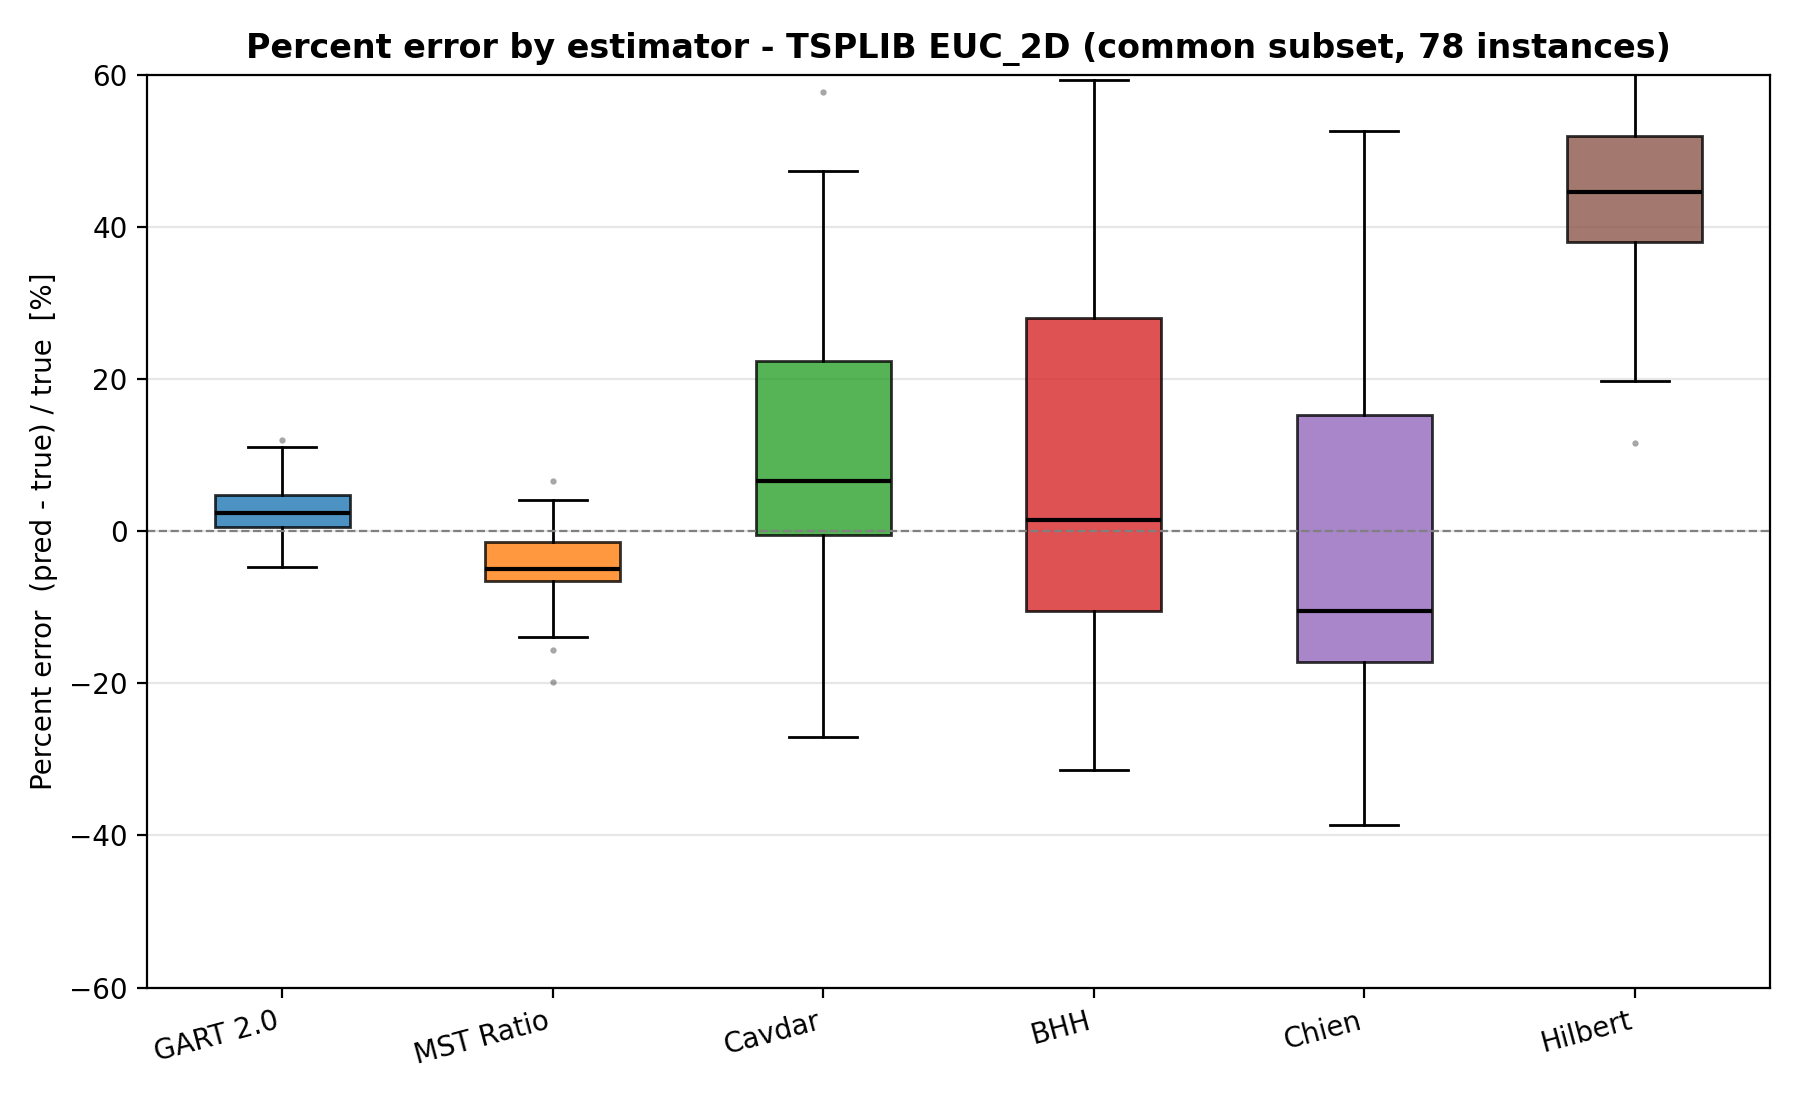
\includegraphics[width=0.75\textwidth]{boxplot_tsplib_errors.png}
\caption{Percent-error distribution per model on the TSPLIB95 EUC\_2D subset (78 instances).}
\label{fig:boxplot_tsplib}
\end{figure}

GART 2.0 transfers from synthetic to real-world at 3.44\% MAPE / 3.52\% SDPE --- tighter than every classical baseline including MST Ratio (5.22\% / 4.54\%). The largest instance ($n = 85{,}900$, 86$\times$ the training cap) is predicted in under 0.5~s. BHH, Cavdar, and Chien all degrade past $n = 500$, where real-world instances violate the uniform-density assumption their derivations require. In the $[2001, 10000]$ and $n > 10000$ buckets MST Ratio matches or beats GART on MAPE (2.70\% vs 5.77\%, 1.85\% vs 2.86\%): true $\alpha$ in large TSPLIB EUC\_2D instances concentrates near the asymptotic value of 1.07--1.15 \citep{percus1996}, so a fixed-constant predictor is hard to beat on accuracy. GART still wins on SDPE in every TSPLIB bucket, which confirms that its per-instance adjustments are informative even when they do not move the mean.

\subsection{Discussion}

Three patterns recur across benchmarks.

\textbf{MST Ratio converges to GART 2.0 at high density.} In the $d = 100$ ND bucket, MST Ratio MAPE is 6.54\% vs GART 0.90\%; in the largest TSPLIB bucket the two estimators agree within 1\% MAPE. The reason is that $\alpha \to 1$ as dimension or density grows \citep{percus1996}, so any fixed constant near 1 becomes a decent approximation. GART's advantage lives in the mid-density regime where $\alpha$ still varies meaningfully with instance topology --- exactly the regime that dominates practical logistics.

\textbf{Geometric estimators are inapplicable in $d \ge 3$.} BHH, Cavdar, and Chien all require the convex hull area or bounding-box volume. Hull computation costs $O(n^{\lfloor d/2 \rfloor})$ \citep{orourke1998} and the hull-to-box volume ratio shrinks exponentially with $d$ \citep{carlsson2024upper}; these baselines are absent from the ND results by construction.

\textbf{Cost structure.} On the TSPLIB log --- the only timing log in our pipeline that cleanly separates preparation from inference --- GART 2.0 spends 74.8\% of wall time on feature extraction and MST construction and 25.0\% on LightGBM inference; classical baselines spend $\ge 99\%$ on feature/MST preparation. GART's overhead relative to a classical baseline is the feature pipeline itself, not the tree ensemble. The pipeline cost is sunk for any MST-based estimator.

Known weak points: grid lattices and near-linear manifolds (Line Noise 10.86\% MAPE in Table~\ref{tab:2d_by_size}), where MST topology becomes structurally degenerate. These cases are rare in real logistics but informative for mapping the model's boundary.

\section{Application: Non-Euclidean Estimation via MDS Embedding} \label{sec:application}

TSPLIB95 contains 32 metric instances that are not native EUC\_2D: 4 CEIL\_2D (Euclidean with ceiling-rounded distances), 2 ATT (pseudo-Euclidean), 10 GEO (great-circle geographic), and 16 EXPLICIT-metric (distance-matrix only). Classical estimators cannot process these: BHH and Cavdar require 2D coordinates, Chien requires convex hull area, and Hilbert requires a Euclidean embedding. We present GART 2.0 as the sole estimator viable on these cases. Timings are reported as an exploration of capability, not a comparison. We exclude the EXPLICIT outlier \texttt{brg180} from every aggregate because its distance matrix has 85{,}368 triangle-inequality violations: GART 2.0 (like any MST-based estimator) assumes symmetric metric distances, so non-metric instances are out of scope for this model.

\subsection{MDS preprocessing}

Classical multidimensional scaling \citep{torgerson1952mds,borg2005mds} embeds an $n \times n$ distance matrix $D$ into $k$-dimensional Euclidean coordinates. Let $J = I - \tfrac{1}{n}\mathbf{1}\mathbf{1}^\top$ be the centering matrix and $D^{(2)}$ the elementwise-squared distance matrix. The doubly-centered inner-product matrix is $B = -\tfrac{1}{2} J D^{(2)} J$; its eigendecomposition $B = V \Lambda V^\top$ yields the embedding $X = V_k \Lambda_k^{1/2}$ on the top $k$ positive eigenvalues \citep{cox2000mds}. We pick the smallest $k$ retaining $\ge 99.9\%$ of the eigenvalue variance, capped at $k = 100$. MST features are computed from the \emph{original} distance matrix (preserving metric accuracy), while geometric features use the embedded coordinates. The selected $k$ is passed to the model as the dimension feature. Appendix~\ref{app:mds} gives the derivation.

\subsection{Results on non-Euclidean TSPLIB95}

\begin{table}[!ht]
\centering
\caption{GART 2.0 on non-Euclidean TSPLIB95 (32 instances). Embedded dimension $k$ is chosen per instance by MDS variance retention.}
\label{tab:tsplib_nonEuc}
\resizebox{\textwidth}{!}{%
\footnotesize
\begin{tabular}{@{}l r r r r r r c@{}}
\toprule
Distance type & $N$ & MAPE (\%) & SDPE (\%) & Median (\%) & $R^2_\alpha$ & Time (ms) & Embed.\ $k$ (avg [range]) \\
\midrule
CEIL\_2D & 4 & 7.11 & 6.54 & 6.96 & $-0.786$ & 581 & 2 [2,2] \\
ATT & 2 & 4.40 & 1.17 & 4.40 & --- & 16.6 & 53 [6,100] \\
GEO & 10 & 4.44 & 2.75 & 4.95 & 0.810 & 16.5 & 16 [2,61] \\
EXPLICIT-metric & 16 & 5.94 & 6.04 & 5.19 & 0.391 & 12.3 & 38 [8,100] \\
\midrule
\textbf{TOTAL} & \textbf{32} & \textbf{5.55} & \textbf{5.32} & \textbf{5.03} & \textbf{0.415} & \textbf{84.7} & --- \\
\bottomrule
\end{tabular}%
}
\end{table}

GART 2.0 generalizes across all four distance types with 4--7\% MAPE. GEO instances achieve the lowest error (4.44\%) because great-circle distances admit a low-stress Euclidean embedding at typical geographic scales. EXPLICIT-metric instances reach 5.94\% because their matrices may mildly violate the triangle inequality, inflating MDS stress. CEIL\_2D runtime is inflated by two of its four instances exceeding $n = 10{,}000$, which dominates the 581~ms mean.

\begin{figure}[!ht]
\centering
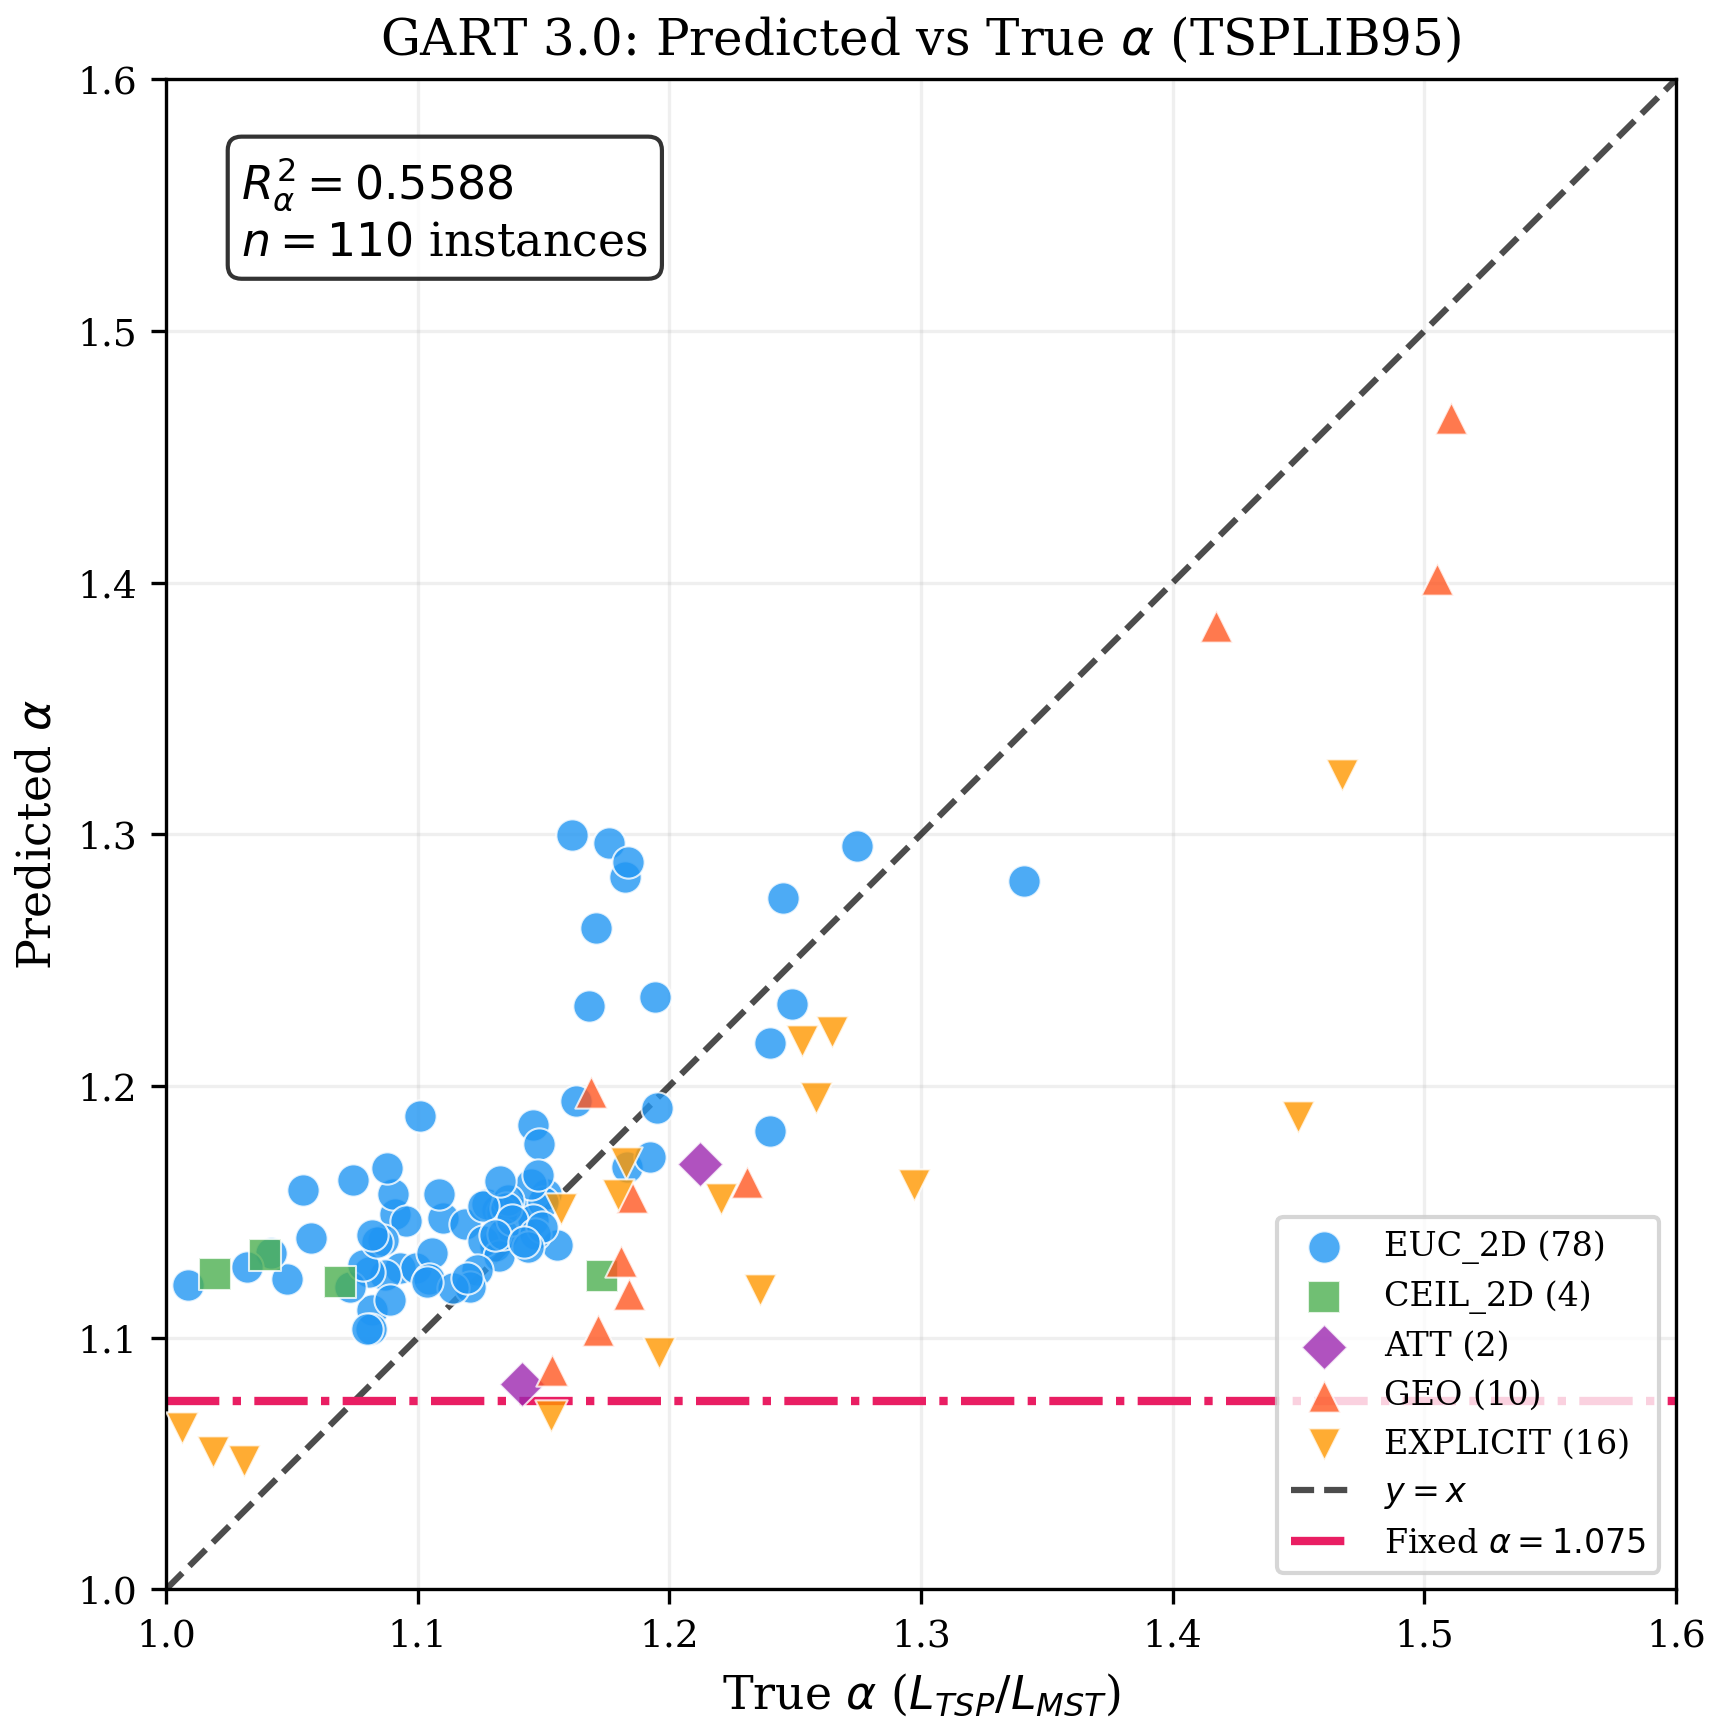
\includegraphics[width=0.75\textwidth]{tsplib_extrapolation.png}
\caption{GART 2.0: predicted vs.\ true $\alpha = L_{\text{TSP}} / L_{\text{MST}}$ on all 110 TSPLIB95 instances, colored by distance type. Combined data from the 78 EUC\_2D instances of Section~\ref{subsec:results_tsplib} and the 32 non-Euclidean instances of Table~\ref{tab:tsplib_nonEuc}.}
\label{fig:tsplib_scatter}
\end{figure}

Figure~\ref{fig:tsplib_scatter} combines all 110 TSPLIB95 metric instances on a single predicted-versus-true $\alpha$ plot. Predictions cluster along the diagonal across every distance type, showing that the MST-to-TSP ratio is learnable even when coordinates are derived rather than native. A pattern worth noting: the non-Euclidean subsets (GEO, EXPLICIT-metric) produce wider true-$\alpha$ spreads than EUC\_2D, so GART 2.0 has more signal to explain --- and indeed $R^2_\alpha = 0.81$ on GEO exceeds the 0.16 on EUC\_2D. On EUC\_2D, most real-world instances converge to $\alpha \in [1.07, 1.15]$; that narrow band leaves little variance for even a good predictor to explain, which drives the low EUC\_2D $R^2_\alpha$ despite the 3.44\% MAPE. The implication is that instances with higher true-$\alpha$ variation are where MST-based prediction has most to contribute, and where the next generation of features should focus.

